\documentclass[12pt]{article}
\usepackage[letterpaper, margin=1in]{geometry}
\usepackage{graphicx}
\usepackage{subcaption}
\graphicspath{{./Figures/}}
\usepackage{hyperref}
\usepackage{parskip}

\title{ELECENG 3CL4 Lab 1}
\author{
    Aaron Pinto \\
    pintoa9 \\
    L02
    \and
    Raeed Hassan \\
    hassam41 \\
    L02
}

\begin{document}

\maketitle
\clearpage

% stuff goes here
\section*{Simulation Environment}
The software used for our simulation environment consisted of Microsoft Windows 10 Education (Version 20H2, OS Build 19042.746), MATLAB R2020b Update 3, and Quanser Interactive Labs Version 2.9. This software was run on a Dell laptop with an Intel Core i7-8550U processor, 8GB of DDR4-3200MHz RAM, Intel UHD Graphics 620 (integrated), and a 256GB SSD.

\section*{Familiarization Exercises} % might change subsection tiles, just leave it like this for now
% name them subsection_voltage and subsection_angle (eg vii_voltage/vii_angle)
% don't worry about the figure placement, it'll probably fix itself once you add more text or i'll fix it later

\subsection*{vii/viii} % base settings
Base settings, proportional gain is 1, no derivative gain
\begin{figure}[h!]
    \centering
    \begin{subfigure}[b]{0.49\textwidth}
        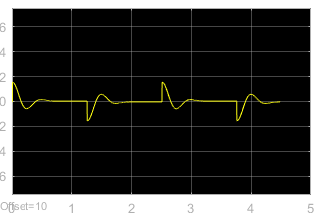
\includegraphics[width=\textwidth]{vii_voltage}    
        \caption{Motor Voltage}    
    \end{subfigure}
    \begin{subfigure}[b]{0.49\textwidth}
        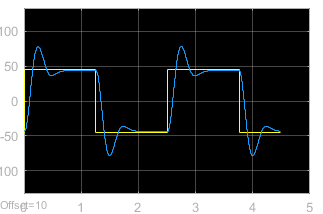
\includegraphics[width=\textwidth]{vii_angle}
        \caption{Servo Angle}
    \end{subfigure}
    \caption{\label{fig:vii} Proportional gain: 1, Derivative gain = 0}
\end{figure}

\subsection*{ix} % increase proportional gain 1 -> 2
Increase proportional gain to 2
\begin{figure}[h!]
    \centering
    \begin{subfigure}[b]{0.49\textwidth}
        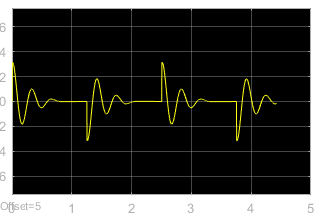
\includegraphics[width=\textwidth]{ix_voltage}
        \caption{Motor Voltage}
    \end{subfigure}
    \begin{subfigure}[b]{0.49\textwidth}
        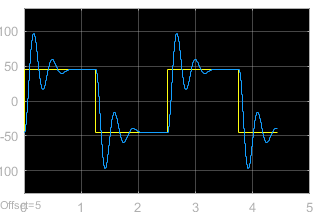
\includegraphics[width=\textwidth]{ix_angle}
        \caption{Servo Angle}
    \end{subfigure}
    \caption{\label{fig:ix} Proportional gain: 2, Derivative gain = 0}
\end{figure}

\subsection*{x} % increase proportional gain 2 -> 4
Increase proportional gain to 4
\begin{figure}[h!]
    \centering
    \begin{subfigure}[b]{0.49\textwidth}
        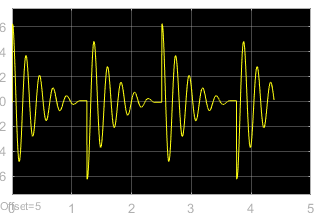
\includegraphics[width=\textwidth]{x_voltage}
        \caption{Motor Voltage}
    \end{subfigure}
    \begin{subfigure}[b]{0.49\textwidth}
        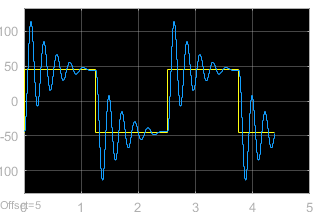
\includegraphics[width=\textwidth]{x_angle}
        \caption{Servo Angle}
    \end{subfigure}
    \caption{\label{fig:x} Proportional gain: 4, Derivative gain = 0}
\end{figure}

\subsection*{xi} % increase derivative gain 0 -> 0.1
Increased derivative gain to 0.1
\begin{figure}[h!]
    \centering
    \begin{subfigure}[b]{0.49\textwidth}
        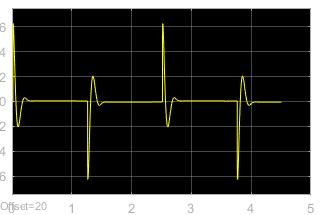
\includegraphics[width=\textwidth]{xi_voltage}
        \caption{Motor Voltage}
    \end{subfigure}
    \begin{subfigure}[b]{0.49\textwidth}
        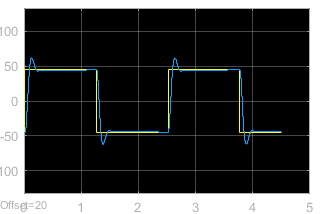
\includegraphics[width=\textwidth]{xi_angle}
        \caption{Servo Angle}        
    \end{subfigure}
    \caption{\label{fig:xi} Proportional gain: 4, Derivative gain = 0.1}
\end{figure}

\subsection*{xii} % increase derivative gain 0.1 -> 0.15
Increase derivative gain to 0.15
\begin{figure}[h!]
    \centering
    \begin{subfigure}[b]{0.49\textwidth}
        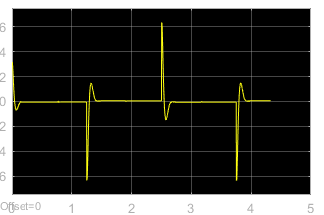
\includegraphics[width=\textwidth]{xii_voltage}
        \caption{Motor Voltage}     
    \end{subfigure}
    \begin{subfigure}[b]{0.49\textwidth}
        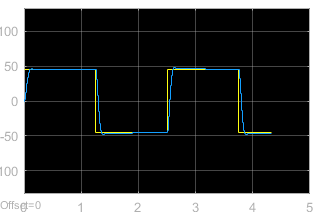
\includegraphics[width=\textwidth]{xii_angle}
        \caption{Servo Angle}
    \end{subfigure}
    \caption{\label{fig:xii} Proportional gain: 4, Derivative gain = 0.15}
\end{figure}

\end{document}
